% -*- TeX-engine: luatex -*-
\documentclass[dvipsnames,presentation,aspectratio=169,14pt]{beamer}
\usepackage{hastingstheme}
\titlegraphic{
\includegraphics[scale=.35]{static_figures/du_bn.pdf}}
\author{\large Massimiliano Fasi}
\date{}

% \usepackage{template}
% \renewcommand{\authorname}{Lawrence Mitchell\inst{*}}
\renewcommand{\authoremail}{\inst{*}\texttt{lawrence.mitchell@durham.ac.uk}}

% \renewcommand{\sessionnumber}{2}
% \renewcommand{\sessiontitle}{Memory hierarchy}


\usetikzlibrary{matrix,fit,positioning,calc}
\usepackage{pgfplots}
% \pgfplotsset{compat=1.15}
\usepackage{pgfplotstable}
% \date{}

\usepackage{tikz}
\usetikzlibrary{matrix,fit,positioning,calc}
\usepackage{pgfplotstable}
\pgfplotsset{compat=1.17}
\usetikzlibrary{pgfplots.groupplots}

\date{}

\begin{document}

\title{\firasemibold\color{White}%
  {\fontsize{20}{0}\selectfont SESSION 3\\
    \fontsize{40}{40}\selectfont Roofline\\models\par}}
\titleslide

\begin{frame}
  \frametitle{Types of resources}

  \begin{columns}
    \begin{column}{0.48\textwidth}
      \begin{block}{Scalable\phantom{g}}
        Scales linearly
        \begin{itemize}[itemsep=6pt]
        \item private resources
        \item floating-point units
        \item CPU cores
        \end{itemize}
      \end{block}
    \end{column}
    \begin{column}{0.48\textwidth}
      \begin{block}{Saturating}
        Scales sublinearly
        \begin{itemize}[itemsep=6pt]
        \item shared resources
        \item L3 memory
        \item RAM
        \end{itemize}
      \end{block}
    \end{column}
  \end{columns}

  \vskip 15pt
  \pause
  \begin{challenge}{Bottlenecks}
    Saturating resources are the limiting factor.
  \end{challenge}

\end{frame}

\begin{frame}
  \frametitle{Scalable vs.~Saturating}
  \begin{columns}
    \begin{column}{0.45\textwidth}
      \begin{tikzpicture}
        \pgfplotstableread[row sep=\\]{%
          Cores Perf\\
          1 1.5\\
          2 3\\
          3 4.5\\
          4 6\\
          5 7.5\\
          6 9\\
          7 10.5\\
          8 12\\}\scaling
        \begin{axis}[xlabel=Cores,
          ylabel=Performance,
          width=\textwidth,height=0.7\textheight]
          \addplot+ table[x=Cores, y=Perf] {\scaling};
        \end{axis}
      \end{tikzpicture}
    \end{column}
    \begin{column}{0.45\textwidth}
      \begin{tikzpicture}
        \pgfplotstableread[row sep=\\]{%
          Cores Perf\\
          1 3\\
          2 6\\
          3 8\\
          4 9\\
          5 9.4\\
          6 9.5\\
          7 9.55\\
          8 9.56\\}\saturating
        \begin{axis}[xlabel=Cores,
          ylabel=Performance,
          width=\textwidth,height=0.7\textheight]
          \addplot+ table[x=Cores, y=Perf] {\saturating};
        \end{axis}
      \end{tikzpicture}
    \end{column}
  \end{columns}
\end{frame}

\begin{frame}[fragile]
  \frametitle{More realistic memory benchmark}
  The \texttt{clcopy} benchmark we used
  \begin{itemize}[itemsep=4pt]
  \item \structure{only} touches one byte in each cache line
  \item \structure{only} provides upper bounds
  \item is not a {realistic} workload
  \end{itemize}

  \vskip 11pt

  State-of-the-art alternative
  \begin{itemize}[itemsep=4pt]
  \item STREAM benchmark\footnote{\url{https://www.cs.virginia.edu/stream/}}
  \item most commonly used is TRIAD
  \item available in \texttt{likwid-bench} as \texttt{stream\_triad\_XXX}
  \end{itemize}
\end{frame}

\begin{frame}[fragile]
  \frametitle{The TRIAD loop}
\begin{minted}{c}
               double *a, *b, *c;
               double alpha = 1;
               ...
               for (int i = 0; i < N; i++)
                  a[i] = b[i]*alpha + c[i];
\end{minted}
  \vskip 11pt
  \pause
  \begin{itemize}[itemsep=5pt]
  \item 2 floating point operations
  \item 2 loads
  \item 1 store
  \end{itemize}
\end{frame}

\begin{frame}
  \frametitle{Code optimisation}
  \begin{center}
    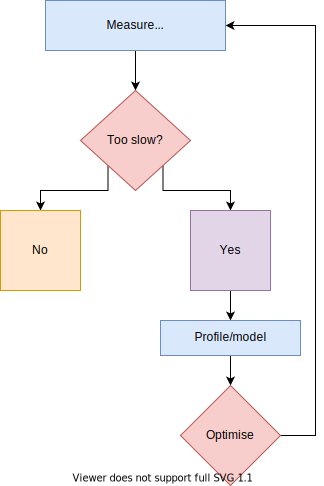
\includegraphics[height=0.8\textheight]{figures/optimisationworkflow.png}
  \end{center}
\end{frame}

\begin{frame}[fragile]
  \frametitle{Simple model for loop heavy code}
  \begin{columns}[t]
    \begin{column}{0.4\textwidth}
      Simple view of \structure{hardware}
      \begin{center}
        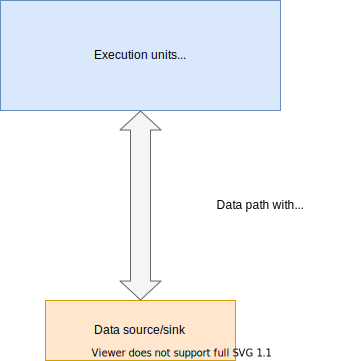
\includegraphics[width=\textwidth]{figures/rooflinecpumodel.png}
      \end{center}
    \end{column}
    \begin{column}{0.5\textwidth}
      Simple view of \structure{software}

\begin{minted}{c}
// Possibly nested loops
for (i = 0; i < ...; i++)
  // Complicated code doing
  // M Flops causing
  // B bytes of data transfer
\end{minted}

      \begin{block}{\small Operational intensity [Flops/B]}
        \begin{equation*}
          I_c = \frac{M}{B}
        \end{equation*}
      \end{block}
    \end{column}
  \end{columns}
\end{frame}

\begin{frame}
  \frametitle{The roofline model \hfill
    \href{https://doi.org/10.1145/1498765.1498785}{\faBook} \ \ \ }
  \begin{challenge}{What is the performance $P$ of a code?}
    How fast can work be done? $P$ measured in Flops/s
  \end{challenge}
  \pause
  \vskip 4pt
  The bottleneck is either:\\[-9pt]
  \begin{itemize}[itemsep=5pt]
  \item execution of work $P_{\text{peak}}$
  \item or the data path $I_c \cdot b_s$
  \end{itemize}
  \vskip 8pt

  Therefore:\\[-11pt]
  \begin{equation*}
    P = \mathsf{min}{(P_\text{peak}, I_c \cdot b_s)}
  \end{equation*}

  \pause
  \vskip 8pt

  \structure{Optimistic model:} everything happens at ``light speed''.

  % Introduced in Williams et al.~\emph{Roofline: An Insightful Visual
  % Performance Model for Multicore Architectures}, CACM (2009).
  % \url{https://doi.org/10.1145/1498765.1498785}
\end{frame}

\begin{frame}
  \frametitle{Roofline diagram}
  \begin{center}
    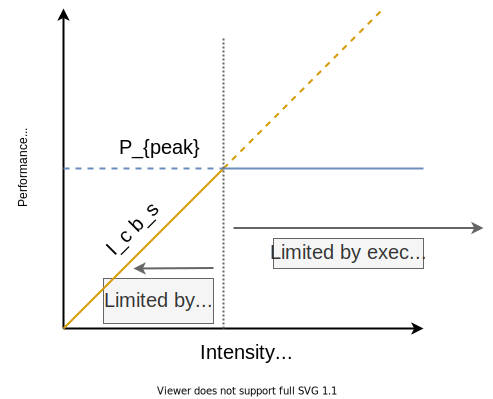
\includegraphics[height=0.8\textheight]{figures/rooflinesketch.png}
  \end{center}
\end{frame}

\begin{frame}
  \frametitle{Applying roofline}
  Roofline characterises performance using three numbers:
  \vskip 6pt
  \begin{enumerate}[itemsep=6pt,leftmargin=60pt]
  \item[\structure{HW1.}] $P_\text{peak}$: peak floating point performance
  \item[\structure{HW2.}] $b_s$: streaming memory bandwidth
  \item[\structure{SW1.}] $I_c$: operational intensity of the code
  \item[\structure{SW2.}] performance of the code
  \end{enumerate}

  \vskip 5pt

  \begin{answer}{Process}
    \begin{enumerate}[wide=0pt]
    \item Measure these numbers
    \item Draw diagram
    \item Use diagram to chose optimisations likely to pay off
    \end{enumerate}
  \end{answer}
\end{frame}

\begin{frame}
  \frametitle{Guide for optimisation choices}
  \vskip -4pt
  \begin{center}
    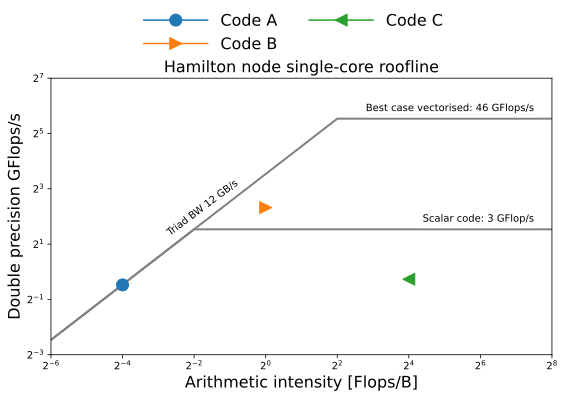
\includegraphics[height=0.78\textheight]{figures/roofline-example-simple.png}
  \end{center}
  \only<1>{\phantom{Wg?}}%
  \only<2>{Which codes might benefit from vectorisation?}%$
  \only<3>{How much improvement could we expect?}%
  \only<4>{Which codes might benefit from refactoring to increase $I_{c}$?}
\end{frame}



\begin{frame}
  \frametitle{Determining the memory bandwidth }
  Data transfers are modeled with \structure{streaming memory bandwidth}

  \begin{exampleblock}{Estimating streaming memory bandwidth (STB)}
    \begin{enumerate}[itemsep=5pt]
    \item \structure{Computation}
      \begin{itemize}[itemsep=3pt]
      \item find out speed of memory $M_{s}$
      \item find out number of memory channels $C$
      \item STB in B/s is $C \times M_{s} \times \mathsf 8$
      \item[\textcolor{Red}{\blacktriangleright}] speed of memory often unknown
        in practice
      \end{itemize}
    \item \structure{Measurement} using STREAM
      \begin{itemize}
      \item typical solution (see exercise 4)
      \end{itemize}
    \end{enumerate}
  \end{exampleblock}
\end{frame}

\begin{frame}
  \frametitle{Determining floating point throughput}
  \structure{Absolute peak} can be estimated from
  \begin{itemize}[4pt]
  \item specification sheet frequency
  \item knowledge of hardware architecture
  \end{itemize}

  \vskip 11pt

  \structure{AMD Zen 2 architecture\hspace{40pt}
    {\footnotesize \href{https://en.wikichip.org/wiki/amd/microarchitectures/zen_2#Floating_Point_Unit}{\faQuestion}}}
  \begin{itemize}[4pt]
  \item Floating point instructions execute on 4 ports
  \item Up to 4 ``$\mu$ops'' issued per cycle
  \item up to 2 floating point instructions per cycle
  \item MUL and FMA ($y \gets a + b\times c$) are issued on ports 0 and 1
  \item ADD are issued on ports 2 and 3
  \item DIV are only issues on port 3
  \end{itemize}
\end{frame}


\begin{frame}
  \frametitle{Example}
  Assuming a maximum clock speed of 3.35GHz

  \vskip 11pt

  \only<1>{%
    \begin{exampleblock}{Example: best case}
      For code with only double precision SIMD FMAs, peak throughput is

      \begin{equation*}
        \overbrace{\mathsf{3.35}}^{\text{clock speed}} \times
        \underbrace{\mathsf 2}_{\text{dual issue}} \times
        \overbrace{\mathsf  4}^{\text{vector width}} \times
        \underbrace{\mathsf 2}_{\text{FMA}} =
        \mathsf{53.6}\text{GFlops/s}
      \end{equation*}
    \end{exampleblock}}\only<2>{%
    \begin{exampleblock}{Example: only DIVs}
      Code only does double precision SIMD DIVs

      \begin{equation*}
        \overbrace{\mathsf{3.35}}^{\text{clock speed}} \times
        \underbrace{\mathsf{1}}_{\text{single issue}} \times
        \overbrace{\mathsf{4}}^{\text{vector width}} =
        \mathsf{13.4}\text{GFlops/s}
      \end{equation*}
    \end{exampleblock}}
\end{frame}

\begin{frame}
  \frametitle{Determining machine characteristics}
  \begin{itemize}[itemsep=8pt]
  \item Sometimes  multiple ``roofs'' for  different instruction mixes
  \item Calculations are complicated by frequency scaling as well
  \end{itemize}

  \vskip 5pt

  \begin{answer}{More details}
    \begin{itemize}[itemsep=5pt]
    \item \url{https://wikichip.org} for spec sheets
    \item \url{https://uops.info} for $\mu$ops execution throughput
    \item \href{https://travisdowns.github.io/blog/2019/06/11/speed-limits.html}
      {Travis Down's discussion} on finding limiting factors in (simple)
      code
    \end{itemize}
  \end{answer}
\end{frame}

\begin{frame}
  \frametitle{Computing operational intensity}
  \structure{Two options:}

  \vskip 6pt

  \begin{enumerate}[itemsep=8pt]
  \item measurement using performance counters
  \item pen-and-paper method
    \vskip 5pt

    \begin{itemize}[itemsep=6pt]
    \item count floating point operations
    \item count data accesses
    \item use formula $I_{C} = M / B$ where
      \begin{itemize}
      \item $M$ is the number of Flops executed
      \item $B$ is the number of bytes moves
      \end{itemize}
    \end{itemize}

  \end{enumerate}

\end{frame}

\begin{frame}[fragile]
  \frametitle{Assessing operational intensity}
\begin{minted}{c}
              double *a, *b, *c, *d;
              ...
              for (i = 0; i < N; i++) {
                a[i] = b[i]*c[i] + d[i]*a[i];
              }
\end{minted}

  \vskip 9pt

  \only<1>{\structure{Counting operations}

    \begin{itemize}
    \item $\mathsf 3$ double-precision Flops/iteration
    \item $\mathsf 3N$ total double-precision Flops
    \item Notice we don't care what operations these are
    \end{itemize}
  }%
  \only<2>{\structure{Counting data accesses}

    \begin{itemize}
    \item Load counts as one access, write as two (one load, one store).
    \item 3 reads, 1 write per iteration.
    \item $\mathsf{8}\times \mathsf{5N}$ total bytes
    \end{itemize}
  }

\vfill
\end{frame}

\begin{frame}[fragile]
  \frametitle{A model of cache}
  \vskip -8pt
  \small

  \begin{columns}[t]
    \begin{column}{0.48\textwidth}
      \begin{solutionblock}{Perfect cache}
        \begin{itemize}[itemsep=0pt, wide=0pt]
        \item Lower bound
        \item Data moved to cache once
        \item Counts \emph{unique} memory accesses
        \item $\mathsf{8\times 2M + 8\times 3N}$ total bytes
        \end{itemize}
      \end{solutionblock}
    \end{column}
    \begin{column}{0.48\textwidth}
      \begin{challenge}{Pessimal cache}
        \begin{itemize}[itemsep=0pt, wide=0pt]
        \item Upper bound
        \item Each array access misses cache
        \item Counts \emph{total} memory accesses
        \item $\mathsf{8 \times 2MN + 8\times 3MN}$ total bytes
        \end{itemize}
      \end{challenge}
    \end{column}
  \end{columns}

  \vskip 13pt

  \begin{itemize}[itemsep=4pt]
  \item These bounds are typically not tight

  \item Better bounds normally require more work in the analysis

  \item Best employed in combination with measurement of operational intensity
  \end{itemize}
\end{frame}

\begin{frame}
  \frametitle{Exercises 4: roofline for matrix-vector multiply}

  \structure{Goal:}

  \begin{equation*}
    y = A x = \sum_{j=1}^{n_{col}} A_{ij} x_j
  \end{equation*}
\end{frame}

\end{document}